% Θεμελιώσεις Κρυπτογραφίας 2016
% Εργασία #1
% Κωσταντίνος Σαΐτας - Ζαρκιάς - 2406
% Οδυσσεύς Κρυσταλάκος - 2362
%-------------------------------------------------------------------------

\documentclass[a4paper, 11pt]{article}


\usepackage[english,greek]{babel} % the last language is the default
	\usepackage[utf8x]{inputenc}

%% > UNCOMMENT if your editor uses iso-8859-7 encoding for Greek (typical in Windows System).
% \usepackage[iso-8859-7]{inputenc}

\usepackage{enumerate}
\usepackage{seqsplit}
\usepackage{hyperref}
\usepackage[pdftex]{graphicx}

\newcommand{\lt}{\latintext}
\newcommand{\gt}{\greektext}
%-------------------------------------------------------------------------

\title{Εργασία 1}

\author{Κωσταντίνος Σαΐτας - Ζαρκιάς - 2406 \\ Οδυσσεύς Κρυσταλάκος - 2362}

\date{\today}

%--------------------------------------------------------------------------
\begin{document}

\maketitle

% ===== Θέμα 1 =====
\section*{Θέμα 1}


\begin{itemize}
	\item[{\lt i)}] Η αρχή του {\lt Kerchoff} υποστηρίζει ότι η ασφάλεια ενός κρυπτοσυστήματος δεν πρέπει να βασίζεται στη γνώση του κρυπτοσυστήματος αλλα στη γνώση του μυστικού κλειδιού. Αναλυτικότερα, σε μία κατάσταση(???) που η Αλίκη προσπαθεί να επικοινωνήσει με τον Μπομπ μέσω ενός μη ασφαλούς δίαυλου η Εύα έχει την δυνατότητα να υποκλέψει τα μηνύματα της Αλίκης αλλά να δεν μπορεί να τα διαβάσει καθώς δεν γνωρίζει το κλειδί με το οποίο έγινε η κρυπτογράφηση στο σύστημα που χρησιμοποίει η Αλίκη και ο Μπομπ.







	\item[{\lt ii)}] Ορισμός τέλειας ασφάλειας κατα {\lt Shannon}: Αν κάποιος έχει ολόκληρο το κρυπτογραφημένο μήνυμα {\lt c}, δεν μπορεί να αποκτήσει καμία πληροφορία για το αρχικό μήνυμα {\lt m}.

					Ορισμός τέλειας ασφάλειας: Ο ορισμός μπορεί να δωθεί και με ένα υποθετικό παράδειγμα στο οποίο η Αλίκη στέλνει ένα μήνυμα {\lt m0} με τέλεια κρυπτογράφηση στον Μπομπ και δίνει στην Εύα το κρυπτογραφημένο μήνυμα {\lt c}, το αρχικό μήνυμα {\lt m0} και ένα άλλο διαφορετικό μήνυμα {\lt m1}. Αν η Εύα δεν μπορεί να ξεχωρίσει το {\lt c} αν προήλθε από το {\lt m0} ή το {\lt m1} και η επιλογή του σωστού βασίζεται σε πιθανότητα ακριβώς 50/50 τότε το κρυπτοσύστημα έχει τέλεια ασφάλεια.







	\item[{\lt iii)}] {\lt XKeyscore}:

	Το {\lt XKeyscore} είναι ένα είδος μηχανής αναζήτησης για τους υπαλλήλους της {\lt NSA} για την συλλογή πληροφοριών ενός στόχου από το ίντερνετ χωρίς την απαίτηση εντάλματος ή κάποιας υπογραφής ανώτερου πολιτειακού στελέχους. Το πρόγραμμα από μόνο του δεν παρεμβάλεται στις επικοινωνίες του στόχου που ορίζει ο χρήστης. Αντίθετα, μαζεύει τις πληροφορίες και υποκλέβει δεδομένα του στόχου από άλλες υπηρεσίες που αναφέρονται παρακάτω.


{\textbf {\lt F6:}} \\
Συνεργασία {\lt CIA} και {\lt NSA} για αποστολές προς ξένους διπλωμάτες και πολιτικούς.

{\textbf {\lt FORNSAT:}} \\
Υποκλοπή δεδομένων από ξένους δορυφόρους.

{\textbf {\lt Overhead:}} \\
Συλλογή δεδομένων από κατασκοπικά αεροπλάνα, {\lt drones} και δορυφόρους.

{\textbf {\lt  SSO (PRISM):}} \\
Συνεργασία {\lt NSA} και ιδιωτικών εταιριών τηλεφωνιάς (π.χ {\lt Verizon}) για την υποκλοπή δεδομένων και τηλεφωνικών συνομιλιών από οπτικες ίνες και κεραίες. Ένα πιο συγκεκριμένο παράδειγμα είναι η επιχείρηση {\lt MUSCULAR} που έχει ως σκοπό την ελεύθερη πρόσβαση της {\lt NSA} στους {\lt servers} της {\lt google} και της {\lt yahoo}.

{\textbf {Επιθέσεις {\lt QUANTUM}}} κινούμενες από το τμήμα {\lt TAO} της {\lt NSA} που ασχολείται κατα κόρον με {\lt cyberwarfare} και {\lt hacking}.

{\textbf {Από άλλες συνεργαζόμενες κυβερνήσεις}} όπως η Αυστραλία, ο Καναδάς, η Νέα Ζηλανδία και το Ηνωμένο Βασίλειο. Η συγκεκριμένη ομάδα αυτών των 5 χωρών μαζί με τις Η.Π.Α είναι γνωστή και ως {\lt Five Eyes} ύστερα από την υπογραφή μυστικής συνθήκης στο τέλος του 2ου Παγκόσμιου Πόλεμου για την μεταξύ τους διάθεση πληροφοριών για κατασκοπία. Ο {\lt Snowden} περιέγραψε την {\lt Five Eyes} ως μια πολυεθνική οργάνωση πληροφοριών που δεν ακολουθεί τους νόμους των χωρών από τις οποίες αποτελείται.
\\

{\textit {Τεχνικές πληροφοριές:}} \\
Διαμοιρασμένο σε μεγάλα {\lt clusters} σε διάφορα σημεία του κόσμου με πάνω από 700 {\lt servers} και έλεγχο περίπου 150 {\lt sites}.

{\textit {Παραδείγματα δυνατοτήτων του προγράμματος:}}
\begin{itemize}

\item Πρόσβαση σε ιστορικό και {\lt mail} οποιουδήποτε.
\item Παρακολούθηση της "κίνησης" ({\lt traffic}) σε οποιουδήποτε {\lt site}.
\item {\lt Real-time} γεωλογικός εντοπισμός φορητών συσκευών με πρόσβαση στο διαδίκτυο.
\item Ακολουθώντας το διαδικτυακό μονοπάτι του στόχου και συλλέγοντας δεδομένα από φόρμες που συμπληρώνει μπορεί να συλλέξει {\lt usernames} και {\lt passwords} για {\lt site} που επισκέπτεται, να βρει την διεύθυνση του στόχου, τους φίλους του και τα ενδιαφέροντά του που τελικώς δημιουργούν ένα ολοκληρωμένο προφίλ ({\lt fingerprint}) μοναδικό για τον κάθε στόχο.

\end{itemize}
\begin{figure}[!ht]
\centering
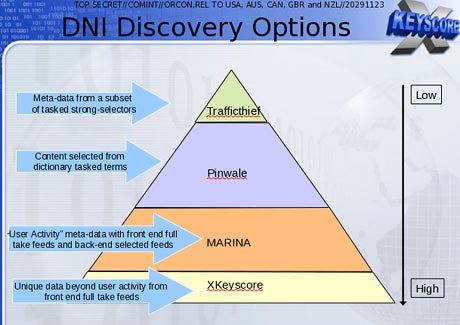
\includegraphics[scale=0.65]{KS10-001.png}
\caption{{\lt Miscellaneous D.N.I (Digital Network Intelligence - intelligence collected by Internet traffic) Software used be NSA and Five Eyes}}
\end{figure}

	% Tempeliko newpage
	\newpage
	\item[{\lt iv)}] Ασφάλεια {\lt OTP}

	Το {\lt OTP} δεν παραμένει ασφαλές αν χρησιμοποιηθεί το ίδιο κλειδί περισσότερες από μία φορές. Αυτό ισχύει για τους παρακάτω λόγους.\\

	Αρχικά, σε περίπτωση που ο επιτηθέμενος, με κάποιον τρόπο, αποκτήσει ένα από τα δύο {\lt plaintext}, μπορεί να αποκρυπτογραφίσει και το άλλο χρησιμοποιώντας το ίδιο κλειδί.\\

	Ακόμη, αν ο επιτιθέμενος αποκτήσει πολλά μηνύματα που έχουν κρυπτογραφηθεί με το ίδιο κλειδί, μπορεί να επιχειρήσει την επίθεση που χρησιμοποιείται και στο κρυπτοσύστημα μετατόπισης. Δηλαδή, μπορεί να βρεί τις συχνότητες εμφάνισης χαρακτήρων και να επιχειρήσει να βρεί το κλειδί. Αυτό ισχύει διότι, χρησιμοποιώντας το ίδιο κλειδί, οι χαρακτήρες των δύο μηνυμάτων που βρίσκονται στις ίδιες θέσεις, έχουν υποστεί την ίδια μετατόπιση.\\

	Τέλος, ο {\lt OTP} είναι ασφαλής ακόμα και ενάντια σε {\lt brute force attacks} καθώς, όλες οι πιθανές περιπτώσεις κλειδιού θα οδηγήσουν σε όλα τα πιθανά μηνύματα. Έτσι, ο {\lt attacker} δεν μπορεί να γνωρίζει το πραγματικό περιεχόμενο. Αν όμως χρησιμοποιηθεί το ίδιο κλειδί, μπορεί να διαπιστωθεί αν ένα πιθανό κλειδί οδηγεί σε πραγματικό κείμενο και για τα δύο κρυπτομηνύματα. Αυτό, αν και δεν δίνει μεγάλο προβάδισμα στον επιτιθέμενο, αυξάνει, έστω και λίγο, τις πιθανότητες να βρεί το αρχικό μήνυμα.

	\item[{\lt v)}] {\lt GCM}

\end{itemize}

\newpage


% ===== Θέμα 2 =====
\section*{Θέμα 2}

Η άσκηση αυτή είχε ως στόχο την δημιουργία του αλγορίθμου κρυπτογράφησης {\lt RC4} και την κρυπτογράφηση ενός μηνύματος.
Επίσης, δημιουργήθηκε μια συνάρτηση αποκρυπτογράφησης για τον έλεγχο της επιτυχής κρυπτογράφησης.

\newpage


% ===== Θέμα 3 =====
\section*{Θέμα 3}
Αρχικά έγινε προσπάθεια εύρεσης του μήκους του κλειδιού που χρησιμοποιήθηκε για την κρυπτογράφηση.
Χρησιμοποιώντας τον δείκτη σύμπτωσης ({\lt Index of Coincidence}) που υλοποιήθηκε σε {\lt Python} και έτσι βρέθηκε
με μεγάλη βεβαιότητα ότι το μήκος του κλειδιού είναι 7 χαρακτήρες ({\lt IC} = 0.06722).
\\
Έτσι το κείμενο διασπάστηκε σε 7 στήλες έτσι ώστε να ισχύει η ίδια μετατόπιση σε κάθε στήλη. Κάνοντας ανάλυση συχνοτήτων
των χαρακτήρων κάθε στήλης, βρέθηκαν οι πιο συχνοί χαρακτήρες κάθε στήλης. Αυτοί είναι:

{\lt
\begin{itemize}
	\item I
	\item Q
	\item T
	\item I
	\item V
	\item S
	\item V
\end{itemize}
}

Αν θεωρηθεί ότι αυτοί οι χαρακτήρες αντιστοιχούν στο {\lt E} (που είναι το γράμμα με την υψηλότερη συχνότητα εμφάνισης), τα
κλειδιά που προκύπτουν σε κάθε στήλη είναι:

\begin{itemize}
	\item Μετατόπιση 4 άρα κλειδί {\lt E}
	\item Μετατόπιση 12 άρα κλειδί {\lt M}
	\item Μετατόπιση 15 άρα κλειδί {\lt P}
	\item Μετατόπιση 4 άρα κλειδί {\lt E}
	\item Μετατόπιση 17 άρα κλειδί {\lt R}
	\item Μετατόπιση 14 άρα κλειδί {\lt O}
	\item Μετατόπιση 17 άρα κλειδί {\lt R}
\end{itemize}

Παρατηρείται ότι σχηματίζουν τη λέξη {\lt EMPEROR} και έτσι φαίνεται πως βρέθηκε το σωστό κλειδί. Με αποκρυπτογράφηση του
μηνύματος με αυτό το κλειδί, προκύπτει το σωστό κείμενο

Αν το κλειδί που προέκυπτε από την παραπάνω ανάλυση ήταν λάθος, θα δοκιμάζονταν άλλοι συνδιασμοί βρίσκοντας τα δεύτερα πιο συχνά εμφανιζόμενα γράμματα κλπ.




\newpage


% ===== Θέμα 4 =====
\section*{Θέμα 4}
Εφόσον χρησιμοποιείται το σύστημα μετατόπισης, τα πιθανά κλειδιά είναι μόλις 23. Επομένως, με επίθεση ωμής βίας μπορούν να
δοκιμαστούν όλα τα πιθανά κλειδιά. Βλέποντας τα αποτελέσματα, παρατηρείται ότι το κείμενο που προκύπτει χρησιμοποιώντας το κλειδί 3 είναι:\\
ΜΗΔΕΙΣΑΓΕΩΜΕΤΡΗΤΟΣΕΙΣΙΤΩΜΟΥΤΗΝΣΤΕΓΗΝ.\\
Αντίθετως, το κείμενα που προκύπτουν από τα υπόλοιπα κλειδιά δεν έχουν κάποιο νόημα. Έτσι έχουμε βρεθεί ότι
το κλειδί είναι 3 και το κείμενο ΜΗΔΕΙΣ ΑΓΕΩΜΕΤΡΗΤΟΣ ΕΙΣΙΤΩ ΜΟΥ ΤΗΝ ΣΤΕΓΗΝ.









\newpage


% ===== Θέμα 5 =====
\section*{Θέμα 5}
Στο θέμα αυτό εξετάστηκε το ποσοστό του {\lt avalanche effect} στον {\lt AES} μεταξύ διαφόρων ζευγαριών μηνυμάτων που διέφεραν μεταξύ τους σε ένα {\lt bit}. Συγκεκριμένα, 32 λέξεις/φράσεις μήκους 16 χαρακτήρων( 16 {\lt bytes} με 5-{\lt bit} κωδικοποίηση μετράπηκαν σε δεκαεξαδικό και ύστερα σε δυαδικά ψηφία και τροποιήθηκε ένα {\lt bit} από την σειρά αυτή δημιουργώντας ένα παρόμοιο μήνυμα. Στην συνέχεια, τα αρχικα και τα τροποποιημένα μηνύματα κρυπτογραφήθηκαν με τον {\lt AES} σε {\lt ECB mode} και {\lt CBC mode} για να εξαταστούν οι διαφορές σε επίπεδο {\lt bit} του κρυπτογραφημένου αρχικού μηνύματος με το κρυπτογραφημένο τροποποιημένο μήνυμα. Η διαδικασία αυτή επαναλήφθηκε για 32 λέξεις/φράσεις και βρέθηκε οτι το ποσοστό μεταλλαγμένων bits σε {\lt ECB mode} ήταν ~50.00 και σε {\lt CBC mode} ήταν 50.00%.




\newpage
% ===== Θέμα 6 =====
\section*{Θέμα 6}

Η μέθοδος που ακολούθησα για την αποκρυπτογράφηση του μηνύματος με οδήγησε στην δημιουργία τριών διαφορετικών μηνυμάτων που προέκυψαν αποκρυπτογραφόντας κάθε φόρα το μήνυμα με ένα από τα γράμματα {\lt K}, {\lt E} και {\lt Y}. Αναλυτικότερα, τα μηνύματα αυτά μπορούν να προκύψουν είτε από συνεχείς αλγεβρικές πράξεις με βάση τον τύπο $ X  Μod 26 - S_{i} $ όπου $S_{i} : i = {K, E, Y} $ είτε με την χρήση του παρακάτω δίσκου σε μια κίνηση.

\centerline{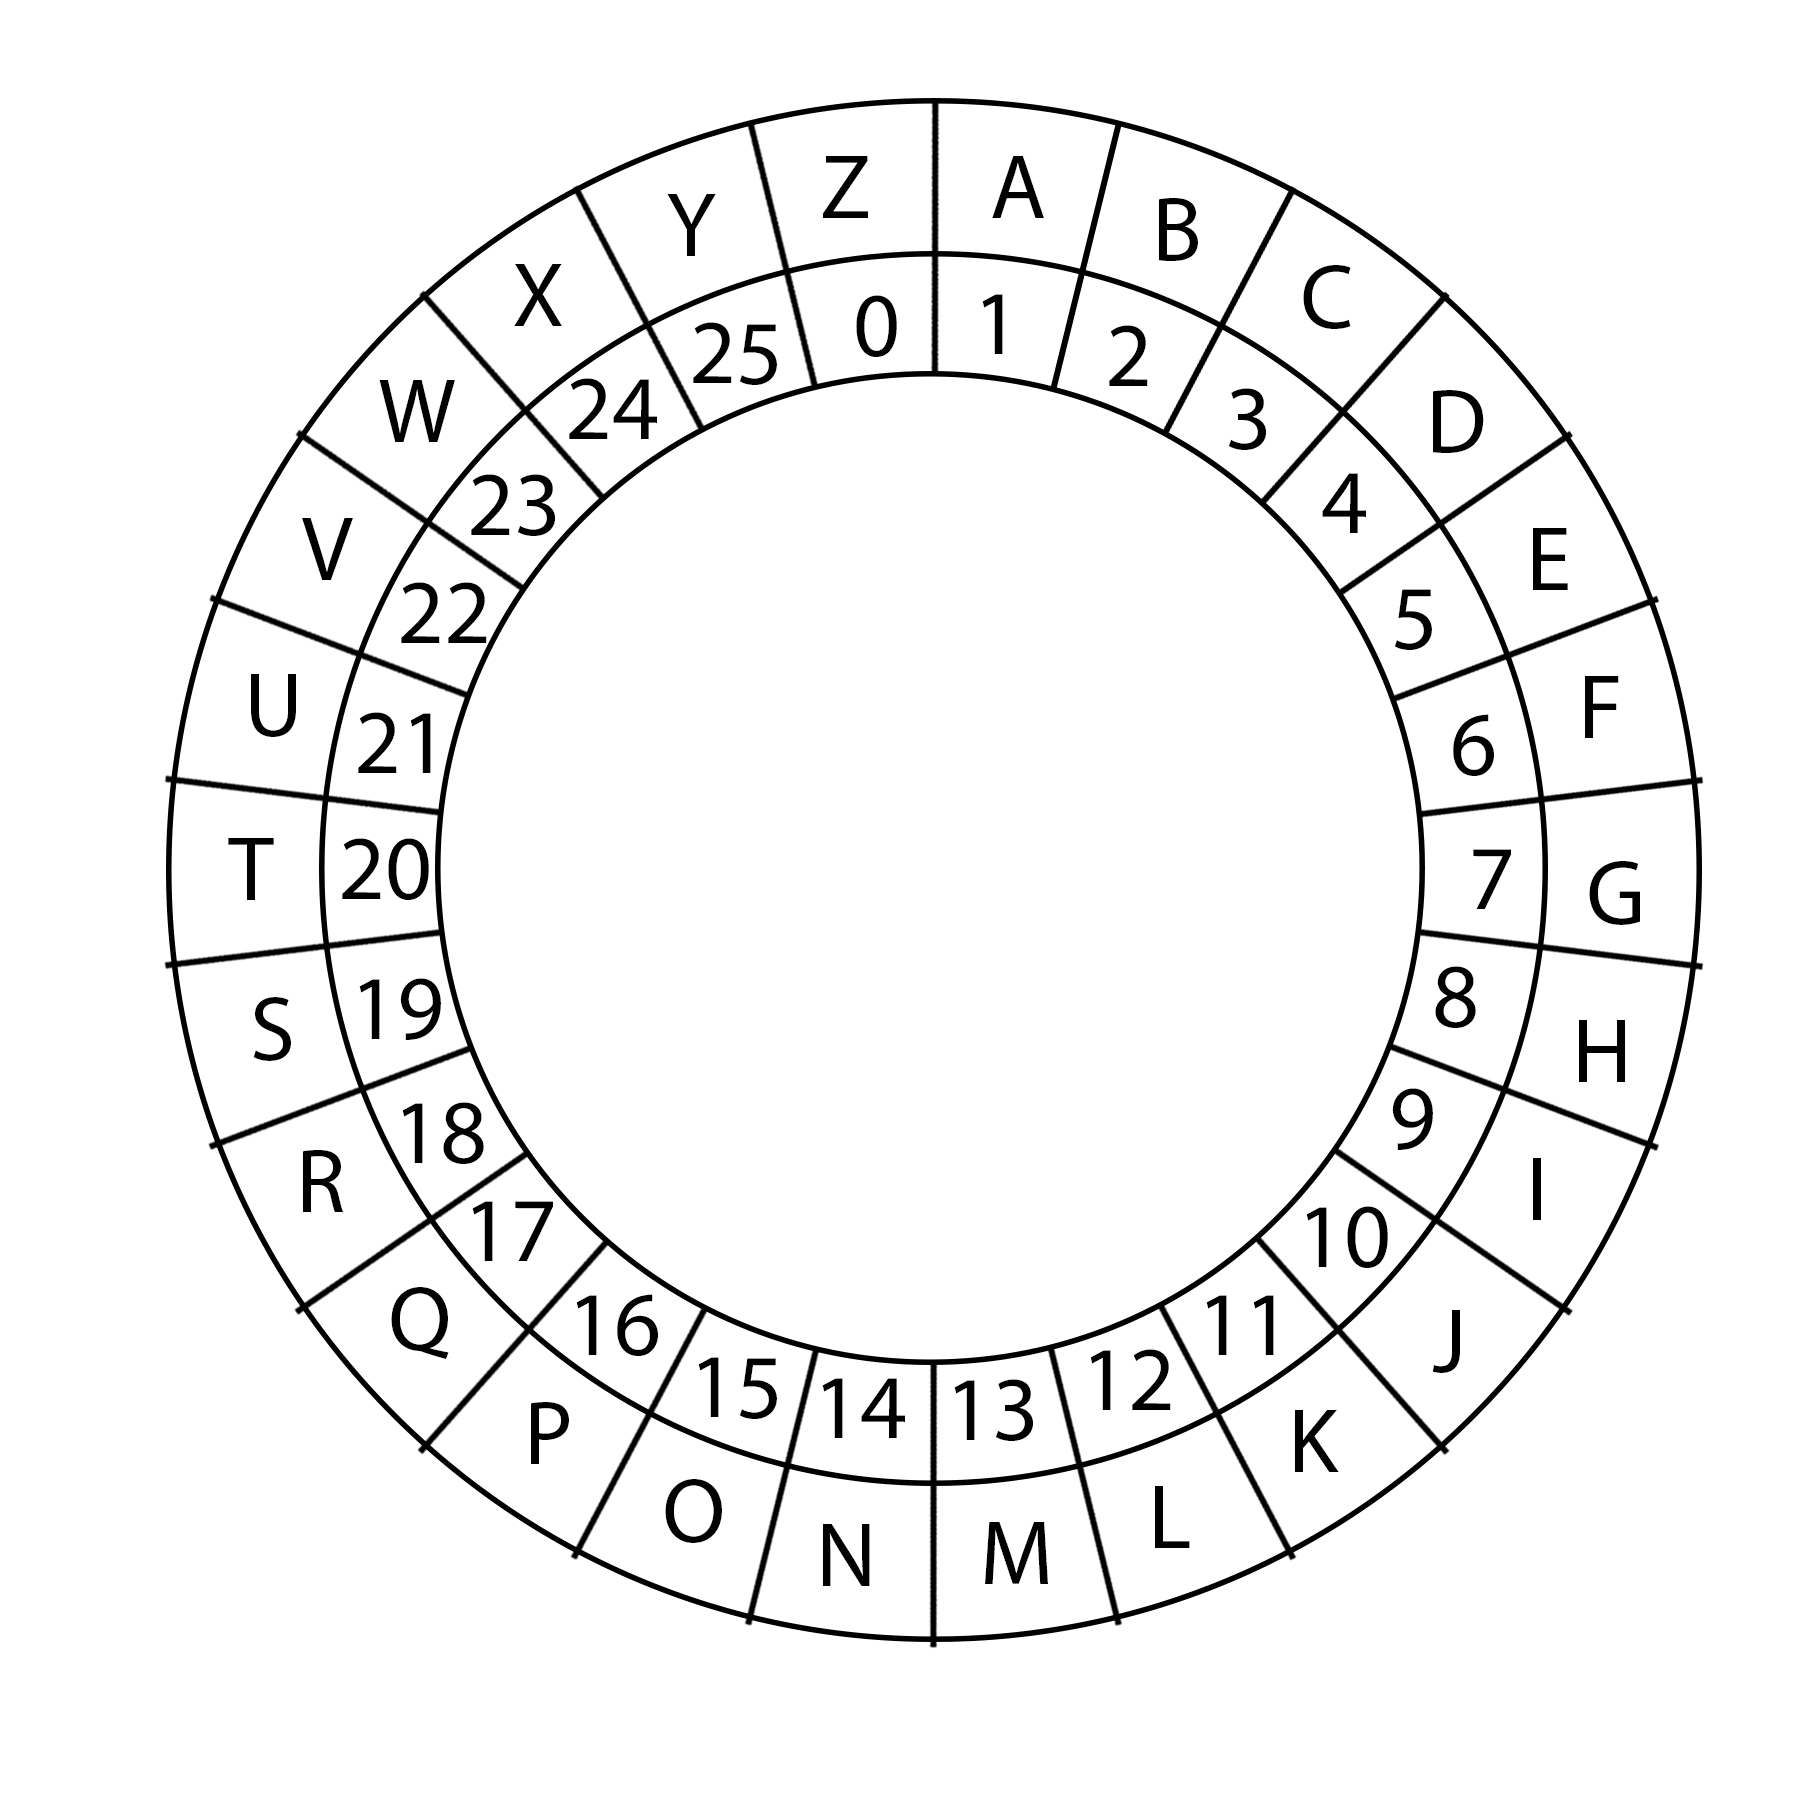
\includegraphics[scale=0.5]{disk.png}}

Ο δίσκος αυτός αναπαριστά το αλφάβητο σε κυκλική μορφή για την διευκόλυνση της εύρεσης του αποτελσματος του {\lt mod26}.
Για παράδειγμα, θέλουμε να αποκρυπτογραφήσουμε το γράμμα Α με βάση το γράμμα Κ.
Αρχικά, σημειώνουμε την θέση του γράμματος Α, δηλαδή το 1, και γυρνάμε τον εξωτερικό δαχτύλιο του αλφάβητου ως ότου το γράμμα με το οποίο αποκρυπτογραφούμε (σε αυτήν την περίπτωση το Κ να έρθει πάνω από τον αριθμό 1. Ύστερα, παρατηρούμε σε ποιόν αριθμό τώρα αντιστοιχεί το γράμμα Α, δηλαδή το 16, και συμβολευόμαστε τον αρχικό δίσκο ποιό γράμμα βρίσκεται σε αυτόν τον αριθμό, δηλαδή το {\lt P}.


\newpage


% ===== Θέμα 7 =====
\section*{Θέμα 7}
Χρησιμοποιήθηκε επίθεση ωμής βίας, δηλαδή δοκιμάστηκαν ως κλειδιά όλες οι λέξεις που βρίσκονται στο {\lt english.txt}. Μετά απο αρκετές προσπάθειες
βρέθηκε το κλειδί: {\lt secret}.



\newpage


% ===== Θέμα 8 =====
\section*{Θέμα 8}
shadow



\newpage


% ===== Θέμα 9 =====
\section*{Θέμα 9}
\subsection*{{\lt (i)}}
Έστω $K$ το {\lt keystream} που χρησιμοποιήθηκε για την κρυπτογράφηση.\\
Έστω $C$ το κρυπτογραφημένο κείμενο.\\
Για να βρεθεί το αρχικό κείμενο ακολουθήθηκε η παρακάτω διαδικασία:\\

Πρώτα, χρησιμοποιώντας το {\lt known plaintext} $ab$ για το κρυπτογραφημένο $sq$, μπορούν να βρεθούν τα {\lt bits} 10-19 του $Κ$.
Αυτό γίνεται κάνοντας {\lt XOR} μεταξύ των 5-{\lt bit} κωδικοποιήσεων των $ab$ και $sq$.

Γνωρίζουμε πως τα {\lt bits} $Κ[10:20]$ που βρέθηκαν, είναι μία ανεστραμμένη κατάσταση του {\lt LFSR} (λόγω της ιδιότητας του {\lt LFSR} να βγάζει
αντίστροφα τα {\lt bits} των καταστάσεων μέσα στο $K$). Συγκεκριμένα γνωρίζουμε ότι τα {\lt bits} $Κ[10:20]$ μας δίνουν την 10 κατάσταση του {\lt LFSR}.\\

\noindent Έστω $S$ η αντεστραμμένη ακολουθία των {\lt bits} 10-19\\

Για να βρούμε το πλήρες {\lt keystream} μπορούν να ακολουθηθούν δύο μεθοδολογίες:

\begin{itemize}
\item Αντίστροφο {\lt LFSR} ξεκινώντας από την κατάσταση 10 μέχρι να βρεθεί το {\lt seed} (κατάσταση 0)
\item Εκτέλεση του {\lt LFSR} με κλειδί τo $S$ και χρησιμοποίηση μόνο ενός τμήματος του {\lt stream}
\end{itemize}

Για λόγους ευκολίας υλοποίησης, χρησιμοποιήθηκε η δεύτερη μεθοδολογία. Αναλυτικότερα, το $Κ$ είναι το τμήμα του {\lt stream} που έχει:\\
\begin{itemize}
\item Έναρξη: 1023 - 10 = 1013 \\(Περίοδος του {\lt LFSR} - μετατόπιση επειδή δόθηκε ως κλειδί η 10η κατάσταση)\\
\item Μήκος: {\lt len(Ciphertext)} * 5 \\(Αριθμός χαρακτήρων του κρυπτογραφημένου * 5 {\lt bit} ανά χαρακτήρα)\\
\end{itemize}

Έτσι προκύπτει το $K$. Κάνοντας {\lt XOR} μεταξύ του $K$ και του $C$, γ́ινεται γνωστό το αρχικό μήνυμα



\end{document}
